\chapter{Discussion}
\label{chap:disc}

\section{Overview}
The approach presented in this study shows a number of strengths. One of the most important strengths of this approach is that it is a trainable one. This means that no prior knowledge is needed, about the application or how the symbols are designed, in the way it operates. Patterns or prototype features, which are used for their configuration are randomly selected. Subsequently, only identical or similar patterns are detected where all parts of the filter defining the selected prototypes' features are present. \\

This makes the approach not just effective for electrical or architectural symbols only but any type of symbol which can be found in various documents, as described in Section \ref{sec:whatis}. This versatility in application is achieved by the application of the COSFIRE filters in various invariance modes. COSFIRE filters can be applied in rotation, scale and reflection invariant mode. Furthermore, COSFIRE filters are not limited to the use of Gabor filters only. Any filter which provides information about contours can be used. \\

The presented approach is effective when applied to datasets with symbols, with both straight lines and curvatures, that included different levels of deformations, different types of noises and different types of geometrical transformations. In most of the datasets that have been processed the recognition rate was higher than that reported in the GREC'11 contest paper. The only datasets which did not surpass the recognition rates reported in the contest paper where the Rotation and RotationScaling datasets. 

\section{Robustness to Scalability}

The best recognition rates for the first category of datasets was achieved with the first 9 experiments, achieving a perfect recognition rate. After those experiments the recognition only decreased slightly, with the lowest recognition of 97.6\%. This decrease in recognition rate is due to the fact that the number of models available for each dataset increases, therefore classification becomes harder. The first 9 datasets in which we achieved a 100\% recognition rate hold 25 or 50 different models while the rest of the datasets hold 100 to 150 different models. Even though the most complex dataset in this category holds the lowest result, over all performance was very good. This shows that our approach is a scalable one, and that if more models are to be added the results remain good.This shows that the approach used in this study is effective for the first category of datasets which contained only deformations. Fig. \ref{fig:cat1results}, shows a summary of the results obtained for the first category of datasets. \\

\begin{figure*}[h]
        \centering
        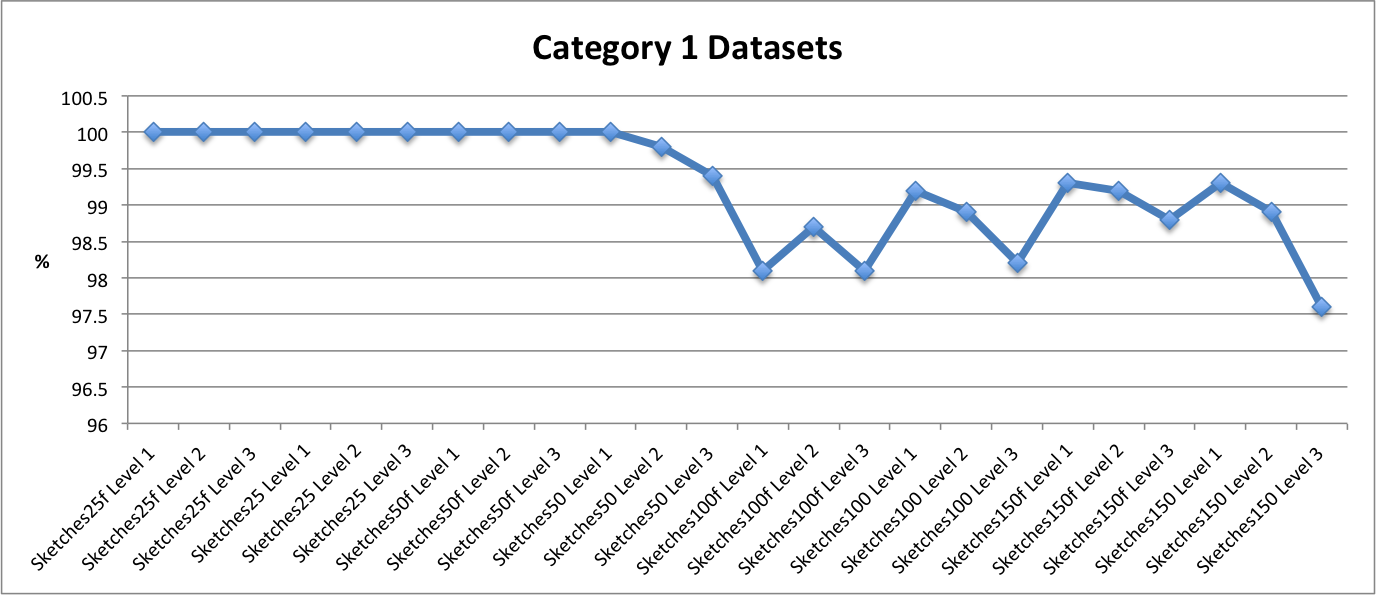
\includegraphics[width=1.0\textwidth]{figures/discussion/results.png}
        \caption[Recognition rates for the first category of datasets]{A graph showing the recognition rates for the first category of datasets}
        \label{fig:cat1results}
\end{figure*}


\section{Robustness to Geometrical Transformations}
The second category of datasets was more difficult due to geometrical transformation such as rotation, scaling or both combined apart from have 150 different models for each dataset. The results show that, Fig.\ref{fig:cat2results}, show that the best performing data set out of this category was the Scaling dataset. The recognition rate achieved with this approached was higher than the recognition rate achieved in the GREC'11 contest. When the rotation transformation was separately introduced in the test images, recognition rates decreased slightly. And the lowest rate was achieved when both scaling and rotation where both introduced in the test image.\\

The drop in recognition rate is due to the number of different orientations chosen at the configuration stage of our approach. Results show that the number of orientations considered was not enough to be able to pick up the rotations introduced in the test images. However even though results have decreased slightly performance remains good which indicates that our approach can also handle geometrical transformations. The following is a  summary of results for the second category of datasets, Fig.\ref{fig:cat2results}.

\begin{figure*}[h]
        \centering
        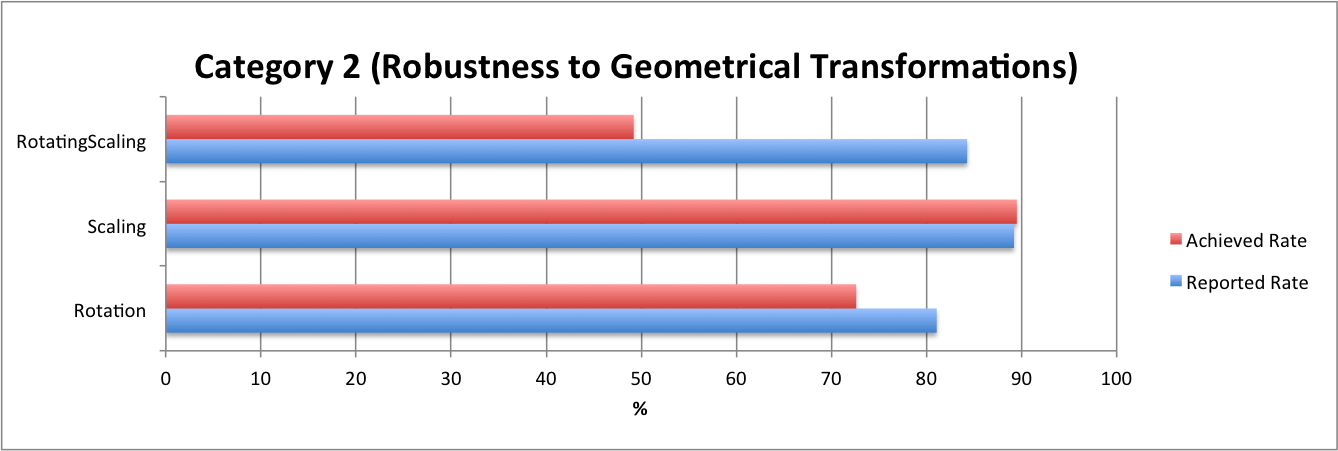
\includegraphics[width=1.0\textwidth]{figures/discussion/results2.png}
        \caption[Recognition rates for the second category of datasets]{A graph showing the recognition rates for the second category of datasets}
        \label{fig:cat2results}
\end{figure*}


\section{Robustness to Noise}
The third category of datasets was also an other difficult category due to added noise and degradations. Also these datasets have 150 different models for each datasets. The recognition rates achieved for these datasets with our approach have surpassed those reported in the GREC'11 contest. A number of pre-processing techniques were applied on the test image prior to classification in order to get rid of noise or enhance the image quality. This shows that our approach is also very robust and efficient when handling noise. The following is a  summary of results for the second category of datasets, Fig.\ref{fig:cat3results}.


\begin{figure*}[h]
        \centering
        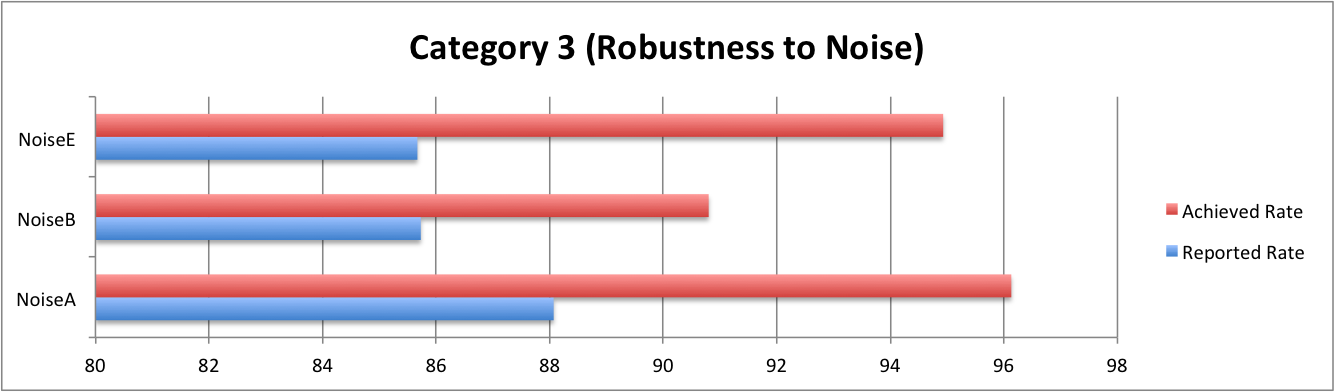
\includegraphics[width=1.0\textwidth]{figures/discussion/results3.png}
        \caption[Recognition rates for the second category of datasets]{A graph showing the recognition rates for the second category of datasets}
        \label{fig:cat3results}
\end{figure*}

\section{Discussion Summary}
In comparison to the approach in their study \cite{Delalandre_2012,Nayef}, the COSFIRE approach achieves robustness to scale, rotation and reflection. In their approach, in order to classify the test image they needed to rotate and scale the model image and create multiple feature vectors describing the same model image. In the approach presented in this study, only one feature vector is needed in order to describe the model image which makes it more efficient due to refraining from working out various feature vectors for each of the models. With this approach we achieved slightly better performance in the scaled datasets. However performance is less for the rotated versions of the datasets.\\ 

We would like to examine and investigate the datasets which contained rotations further. The drop in recognition rate might be due to the fact that the list of of orientations used during configuration is not sufficient. Therefore, we would like to extend further, the experiments presented in this study by considering more rotations. \\

In this approach we do not evaluate the effectiveness of the configured COSFIRE filters.  Since we do not evaluate the resultant operators there is a probability that two operators for two different model symbols might be very similar. This can be due to the fact that any two symbols can have similar geometric primitives. This can be countered by choosing a small subset of test images for evaluation.  \\

Also, in this approach configuration of filters was done randomly by choosing patterns without any attempt at optimisation. Optimisation can be done by altering the COSFIRE filter's parameters in order to discriminate more between any two symbols. One example is the of concentric circles which are used in the configuration. By first analysing such parameters and by subsequently evaluating the attained COSFIRE operators before actually using them would increase the discriminative power during the classification phase.\\